\documentclass{beamer}
\usepackage{graphicx}
\usepackage{paralist}
\usepackage{outlines}

\title{Colour Replacement}
\author{Mendocino College - Digital Image Manipulation with Photoshop}
\titlegraphic{\vspace{-10mm}
\includegraphics[width = .9\textwidth]{images/photoshop.jpg}} 
\date{\vspace{-5em}} 


\mode <presentation>
\usetheme{Warsaw}
\usecolortheme{default}

\setbeamerfont{footline}{size=\fontsize{5}{8}\selectfont}

\definecolor{darkred}{rgb}{20,0,0}
\definecolor{darkgreen}{RGB}{40,110,20}
\definecolor{darkpurple}{RGB}{30,0,30}
\definecolor{chardonnay}{RGB}{255, 255, 204}

\setbeamercolor*{palette primary}{fg=white, bg=darkgreen}


\begin{document}
	{
		\setbeamertemplate{footline}{} 
		\setbeamertemplate{headline}{} 
		\begin{frame}
			\vspace{-35pt}
			\maketitle
		\end{frame}
	}

		\section{Color Replacement Tool}
			\subsection{Color Replacement Tool}		
			\begin{frame}
				\frametitle{The Color Replacement Tool}
				\begin{columns}
					\column{.6\textwidth}
					\vspace{-25pt}
					\begin{outline}
						\1 The Color Replacement tool paints over a targeted color with a replacement color. 
						\1 good for quick edits, it often proves unsatisfactory, particularly with dark colors and black. 
						\1 Uses a foreground color to replace the unwanted color.
					\end{outline}
					\column{.45\textwidth}
					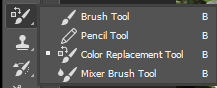
\includegraphics[width=0.9\textwidth]{images/color replacement tool.png}
				\end{columns}
			\end{frame}

		\section{Replace Color Dialog Box}
\subsection{Replace Color Dialog Box}		
\begin{frame}
	\frametitle{Replace Color Dialog Box}
					\begin{outline}
		\1 The Replace Color dialog box combines tools for selecting a color range with HSL sliders for replacing that color.
		\1 Replace Color lacks the Colorize option from the Hue/Saturation adjustment, which may be needed for a complete color change. 
		\1 The Replace Color command is good for global color changes, especially changing out-of-gamut colors for printing.
	\end{outline}
\begin{center}
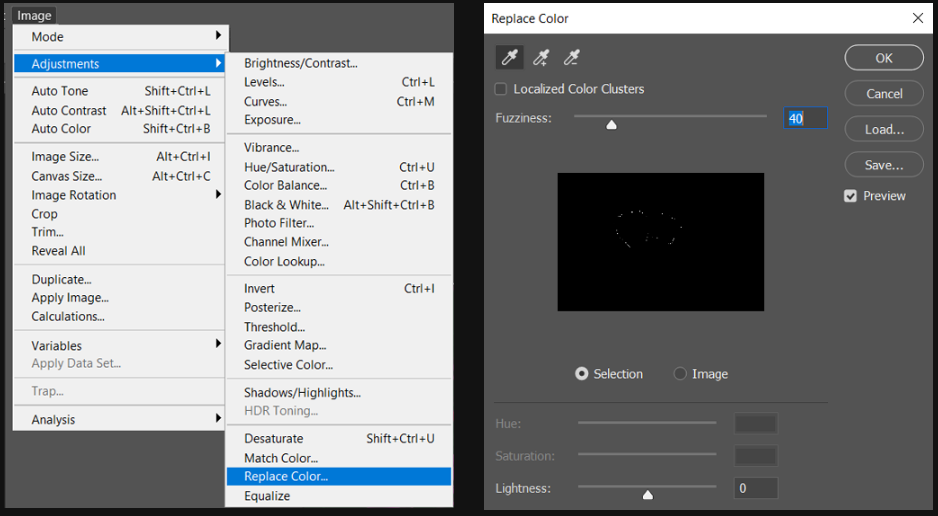
\includegraphics[width=0.55\textwidth]{images/replace color dialog box.png}
\end{center}
\end{frame}

	\section{Hue/Saturation}
			\subsection{Hue/Saturation}		
	\begin{frame}
		\frametitle{Hue/Saturation}
			\begin{columns}
			\column{.6\textwidth}
			\vspace{-25pt}
				\begin{outline}
					\1 Use masks and adjustment layers for non-destructive color replacement.
					\1 This is a flexible technique, allowing you to later fine-tune the results with complete freedom.
				\end{outline}
			\begin{center}
			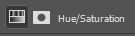
\includegraphics[width=0.5\textwidth]{images/hue saturation.png}
			\end{center}
			\column{.45\textwidth}
				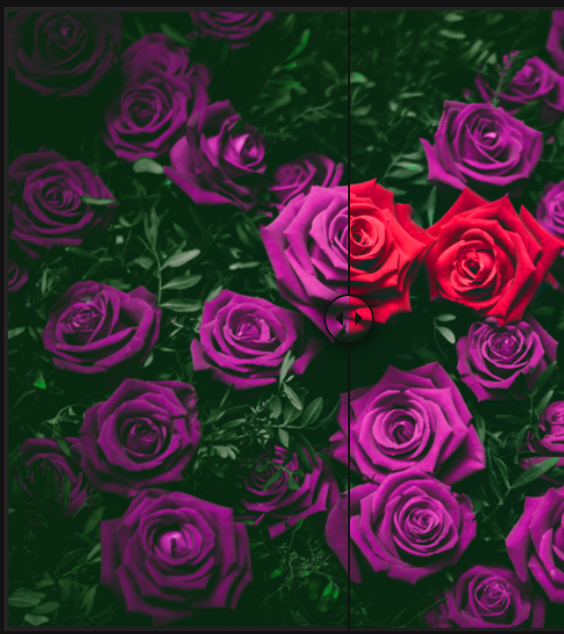
\includegraphics[width=1.0\textwidth]{images/replace color hue.png}
			\end{columns}
		\end{frame}
	
			\subsection{How to use Hue/Saturation adjustment layers}		
				\begin{frame}
					\frametitle{Using Hue/Saturation adjustment layers to change colours.}
									\begin{outline}
						\1 Select the object you wish to change (optional)
						\1 Create a Hue/Saturation Adjustment Layer
						\1 Adjust the Hue slider
					\end{outline}
				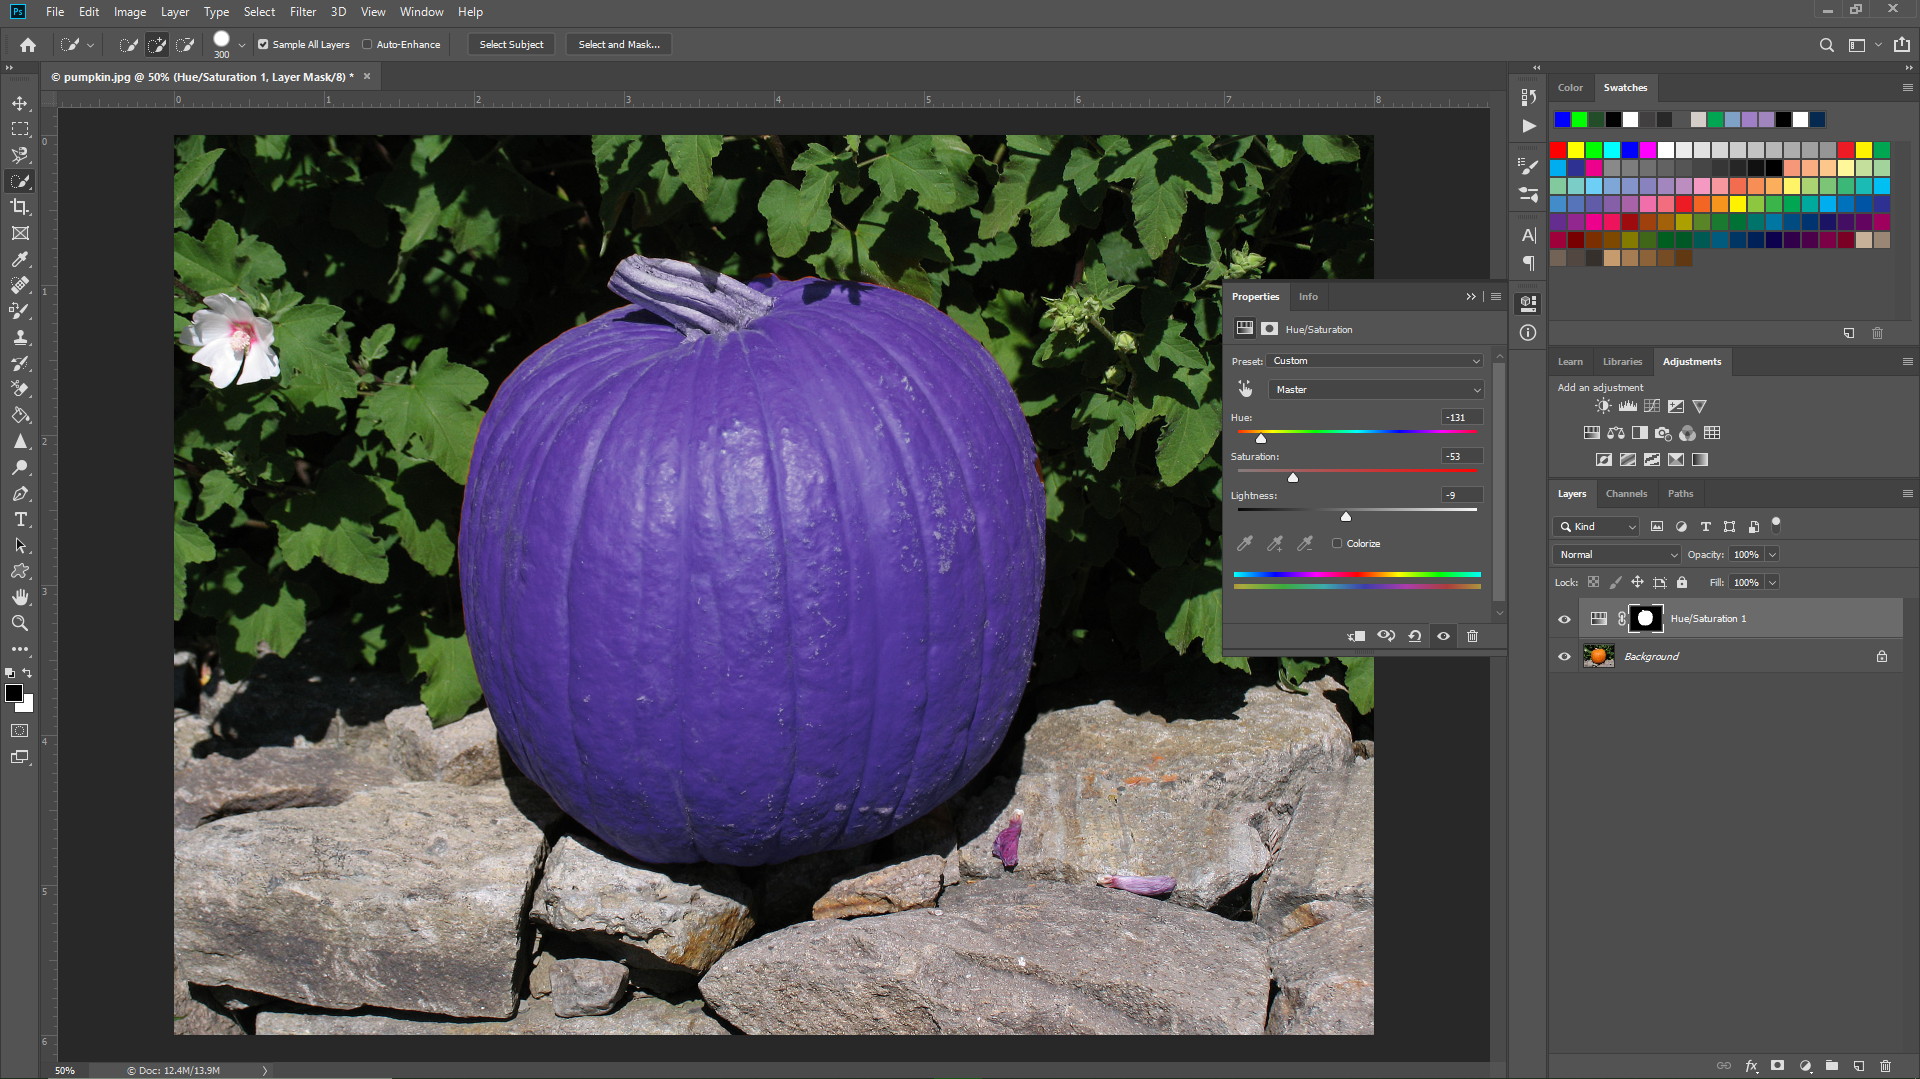
\includegraphics[width=1.0\textwidth]{images/changing color with huge.png}
				\end{frame}

	
	
\end{document}